%Die Angabe des schlauen Spruchs auf diesem Wege funtioniert nur,
%wenn keine Änderung des Kapitels mittels den in preambel/chapterheads.tex
%vorgeschlagenen Möglichkeiten durchgeführt wurde.
%\setchapterpreamble[u]{%
%\dictum[Albert Einstein]{Probleme kann man niemals mit derselben Denkweise lösen, durch die sie entstanden sind.}
%}
\chapter{Implementierung}
\label{chap:impl}
Großer Teil der Arbeit war neben der mathematischen Ausarbeitung (siehe \autoref{chap:maths}) auch die eigentliche Implementierung des erarbeiten Verfahrens, für welche folgende grundlegende Anforderungen bestanden:

\begin{description}
\item[Portierbarkeit:] In der Aufgabenstellung war bereits gefordert, dass die Implementierung auf verschiedenen Systemen portierbar sein soll. Aus diesem Grund kamen bereits nur einige wenige Programmiersprachen in Frage
\item[Evaluation der Daten:] Da die entstehenden Daten auch evaluiert und grafisch dargestellt werden sollten, war eine weitere Anforderung an die Software, dass sie eine \gls{GUI} besitzt oder aber Bild-Formate exportieren kann.
\item[Funktionalität:] Die Funktionalität der Implementierung stand primär im Vordergrund. An die Performanz der Implementierung und dem Design der \gls{GUI} wurden keine besonderen Anforderungen gestellt.
\item[Software-Qualität:] Da diese Arbeit eine Bachelor-Arbeit der Fachrichtung \textit{Softwaretechnik} ist bestand eine gewisse Anforderung an die Qualität des Quellcodes. Dies beinhaltet u.a. automatisierte Tests, Objektorientierte Programmierung und Modulare Strukturen.
\end{description}

\section{Wahl der Programmier-Sprache}
\label{sec:language}
Aus den oben beschriebenen Anforderungen ließen sich im großen und ganzen drei mögliche Programmiersprachen ableiten, aus denen eine gewählt werden musste. In die engere Auswahl kamen dabei \texttt{C}, \texttt{C\#} und \texttt{Java}. Aus \autoref{tab:languages} geht hervor, dass alle diese drei Programmiersprachen für den Einsatzzweck dieser Arbeit geeignet wären. Keine der Sprachen erfüllt ein Kriterium gar nicht oder ragt in einem Bereich besonders hervor. Lediglich \texttt{C} verliert durch die wenige Unterstützung von Software-Qualitätsmerkmalen (wie Objektorientierte-Programmierung, Modularität, Klassen, etc.) an Punkten.

\begin{table}
  \begin{center}
    \begin{tabular}{l|c|c|c|}
	\toprule
      Sprache & \texttt{Java} & \texttt{C} & \texttt{C\#} \\ 
      \midrule
      Portierbarkeit & \checkmark & \checkmark & \checkmark \footnote{Mono (\url{http://www.mono-project.com}) ist eine portierbare Version von C\# die auch auf Unix kompiliert}\\
      \gls{GUI} & \checkmark & \checkmark\footnote{Durch Libraries (z.B. GTK+ \url{http://www.gtk.org}) können in C auch grafische Benutzeroberflächen entwickelt werden } & \checkmark\\
      Objektorientierte Programmierung & \checkmark & $\times$\footnote{Obwohl C keine objektorientierte Sprache ist, ist es grundsätzlich natürlich trotzdem möglich ähnliche Konstrukte zu erzeugen.}  & \checkmark\\
      Automatisierte Tests & \checkmark & \checkmark\footnote{Nicht direkt unterstützt, aber es gibt Testframeworks wie z.B. \url{http://check.sourceforge.net}} & \checkmark\\
      Nativer Systemzugriff\footnote{Der Zugriff auf native Systemfunktionen ermöglicht häufig einen Performance-Gewinn}& $\times$\footnote{Java läuft im sog. \gls{JRE} und hat damit nicht direkt Zugriff auf native Funktionen} & \checkmark & \checkmark\\
	\bottomrule
    \end{tabular}
    \caption{Vergleich der Programmiersprachen \texttt{Java}, \texttt{C} und \texttt{C\#} mit den Anforderungen.}
    \label{tab:languages}
  \end{center}
\end{table}

Da ich selbst bereits mehrere universitäre Projekte mit \texttt{Java} entwickelt habe und mir diese Sprache am besten liegt, entschloss ich mich daher diese für die Implementierung des Algorithmus zu verwenden. 

Für die grafische Evaluation der Ergebnisse entschied ich mich für eine \texttt{SWING}-Oberfläche, die sowohl die Eingabe der Parameter und Daten sowie die Ausgabe der verschiedenen Diagramme und Bilder ermöglichen soll.

Die \autoref{fig:tool} zeigt die einfach gehaltene Oberfläche mit den möglichen Einstellungen.

\begin{figure}
  \begin{center}
    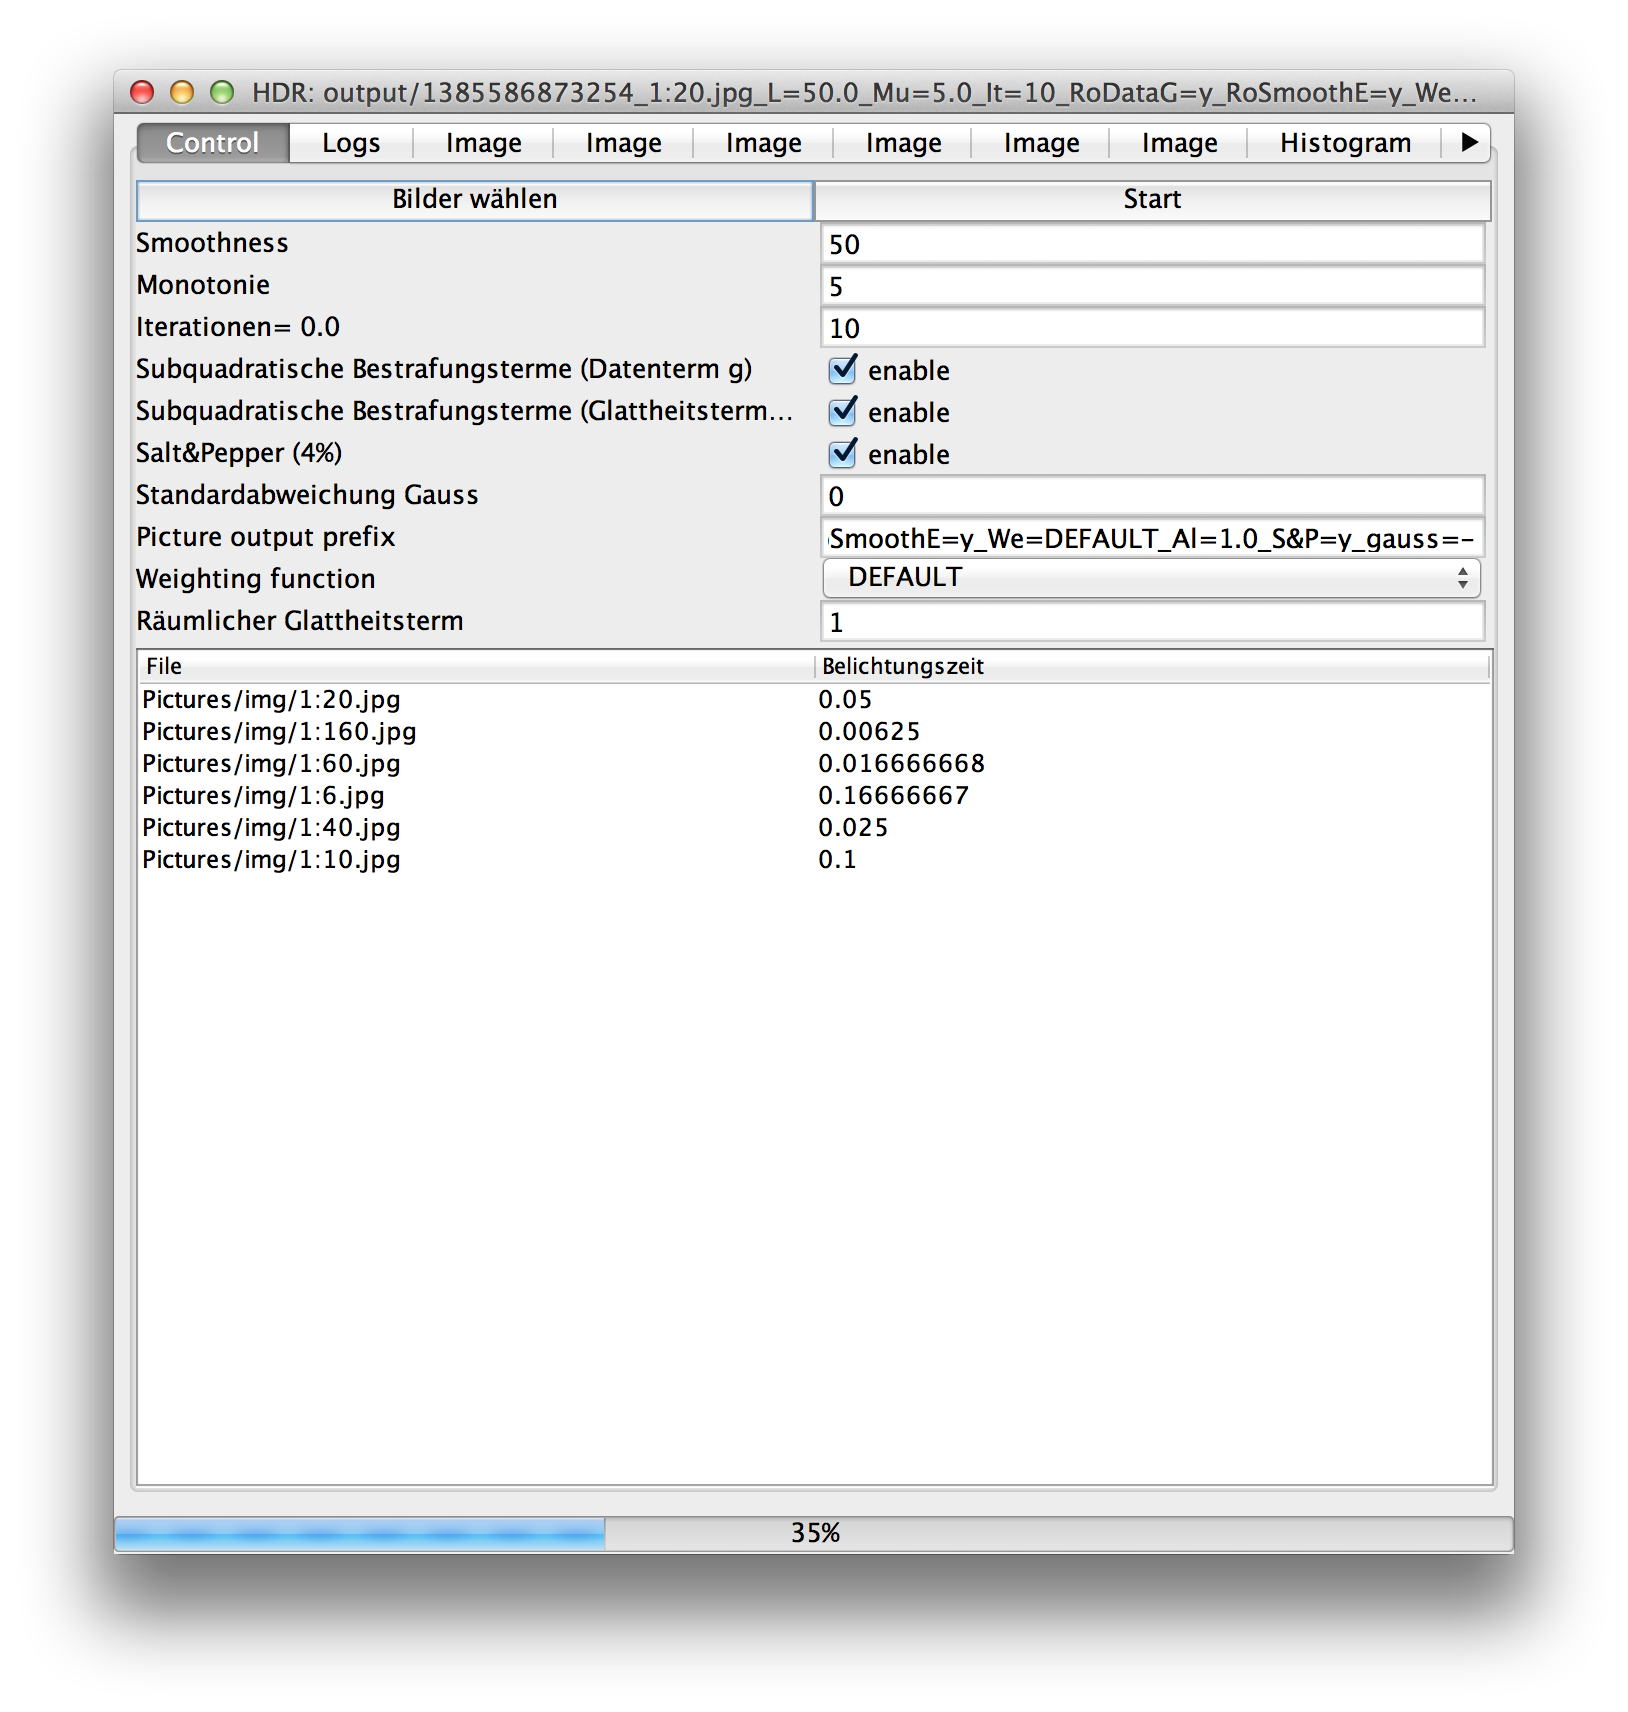
\includegraphics[width=\textwidth]{Tool}
    \caption{Die absichtlich schlicht und pragmatisch gehaltene Benutzereingabe für die Erzeugung der HDR-Bilder.}
    \label{fig:tool}
  \end{center}
\end{figure}


\section{Externe Bibliotheken}
Für die Implementierung wurden einige bereits bestehenden Komponenten eingesetzt. Diese werden hier kurz beschrieben.

\subsubsection*{\texttt{NumericTextField}\footnote{\url{http://www.java2s.com/Code/Java/Swing-JFC/NumericTextField.htm}}}
Für die Eingabe der einzelnen Parameter wird eine Implementierung eines numerischen Textfeldes verwendet. Dieses verhindert ungültige Eingaben und erleichtert das Auslesen der numerischen Parameter.

\subsubsection*{\texttt{metadata-extractor}\footnote{\url{https://code.google.com/p/metadata-extractor/}}}
Die Bibliothek \texttt{metadata-extractor} wird verwendet um automatisiert aus Bilddateien die Belichtungszeit der Bilder auszulesen. Mit ihm wird auch das von Adobe entwickelte \texttt{xmp-core}\footnote{\url{http://www.adobe.com/devnet/xmp.html}} mit geliefert. Zusammen genommen ermöglicht die Bibliothek die Belichtungszeiten der Bilder auszulesen und darzustellen.

\subsubsection*{\texttt{JImageChooser} \footnote{\url{http://docs.oracle.com/javase/tutorial/uiswing/examples/components/index.html\#FileChooserDemo2}}} 
Der verwendete \texttt{JFileChooser} zur Selektion von Bilddateien (und nur diesen) ist inspiriert von dem vorhandenen Tutorial bei Oracle. Er ist in der Lage eine kleine Vorschau der Bilder anzuzeigen.


\section{Architektur}
\label{sec:architektur}
Bei der Architektur der Software wurde eine \gls{MVC} Struktur eingehalten. Dieses Pattern beschreibt eine klare Trennung zwischen Datendarstellung, -verarbeitung und -repräsentation. Diese Teilung in drei Schichten sorgt dafür, dass die einzelnen Komponenten gut getestet werden können und beliebig austauschbar sind. Dadurch besteht ein hoher Grad an Erweiterbarkeit, da die Kopplung zwischen den Modulen möglichst gering gehalten wird.



\subsection{Komponentendiagramm}
Die Anwendung lässt sich grundsätzlich in fünf verschiedene Komponenten trennen (siehe \autoref{fig:arch:components}). 
\begin{description}
\item{\texttt{View}:} Das Paket \texttt{View} behandelt die gesamte Darstellung der Anwendung und die grafische Auswertung der berechneten Bilder. Es enthält \gls{Tone-Mapping} Operatoren und behandelt die Benutzereingabe.
\item{\texttt{Model}:} Das \texttt{Model} besteht in erster Linie aus den Beiden Klassen \texttt{Image} und \texttt{HDRResult}. Erstere wird als Repräsentation eines Bildes verwendet und speichert Grauwerte, Belichtungszeiten und weitere Bildrelevante Informationen. Letztere dient als Kommunikationspaket zwischen dem eigentlichen \texttt{Solver} und der restlichen Anwendung und enthält die fertig berechnete Antwortkurve und die \gls{Radiance Map}.
\item{\texttt{Ctrl}:} Dieses Paket dient zur Steuerung der Anwendung. In diesem werden die Eingaben verarbeitet, an die Algorithmen weiter gegeben und anschließend wieder dargestellt.
\item{\texttt{Maths}:} Die \texttt{Maths}-Komponente enthält alle notwendigen mathematischen Berechnungen und Repräsentationen, wie z.B. \texttt{Matrix} und \texttt{Vector}.
\end{description}

\begin{figure}[H]
  \begin{center}
    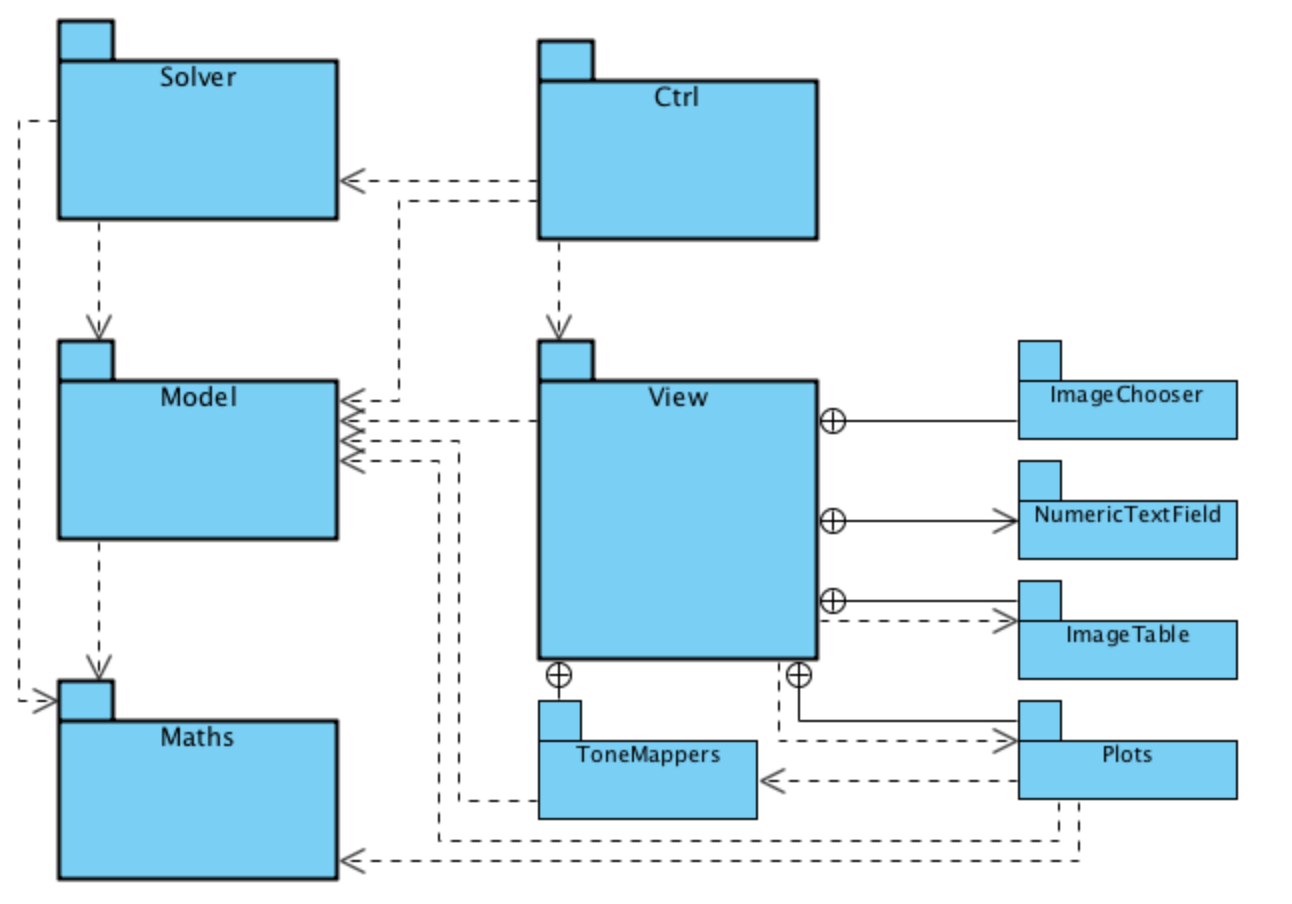
\includegraphics[width=0.8\textwidth]{architecture/components}
    \caption{Die Architektur der Software auf Komponentenebene. Hier kann gut die Trennung zwischen den einzelnen Bereichen erkannt werden.}
    \label{fig:arch:components}
  \end{center}
\end{figure}


\begin{figure}[H]
  \begin{center}
    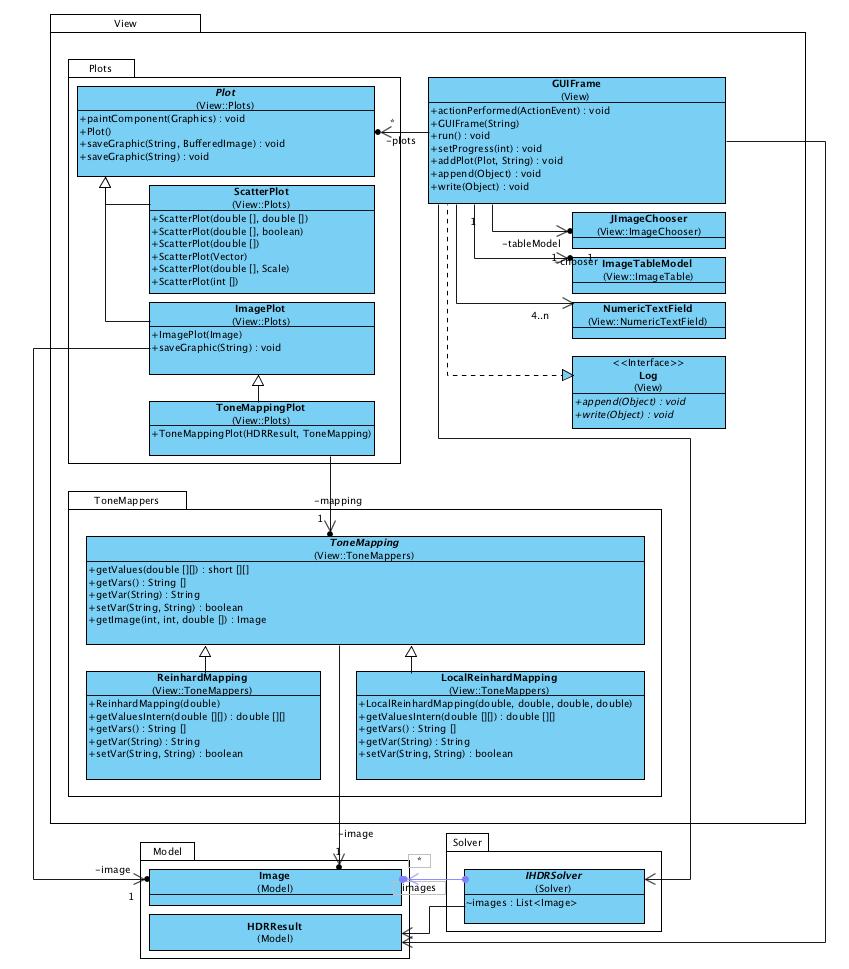
\includegraphics[width=0.8\textwidth]{architecture/view}
    \caption{Die \texttt{View}-Komponente im Detail. Das Hauptfenster \texttt{GUIFrame} stellt die Daten dar und importiert dazu die verschiedenen Komponenten. Die \texttt{Plots} und die \texttt{ToneMappers} gehören ebenfalls zu diesem Paket.}
    \label{fig:arch:plots}
  \end{center}
\end{figure}


\begin{figure}[H]
  \begin{center}
    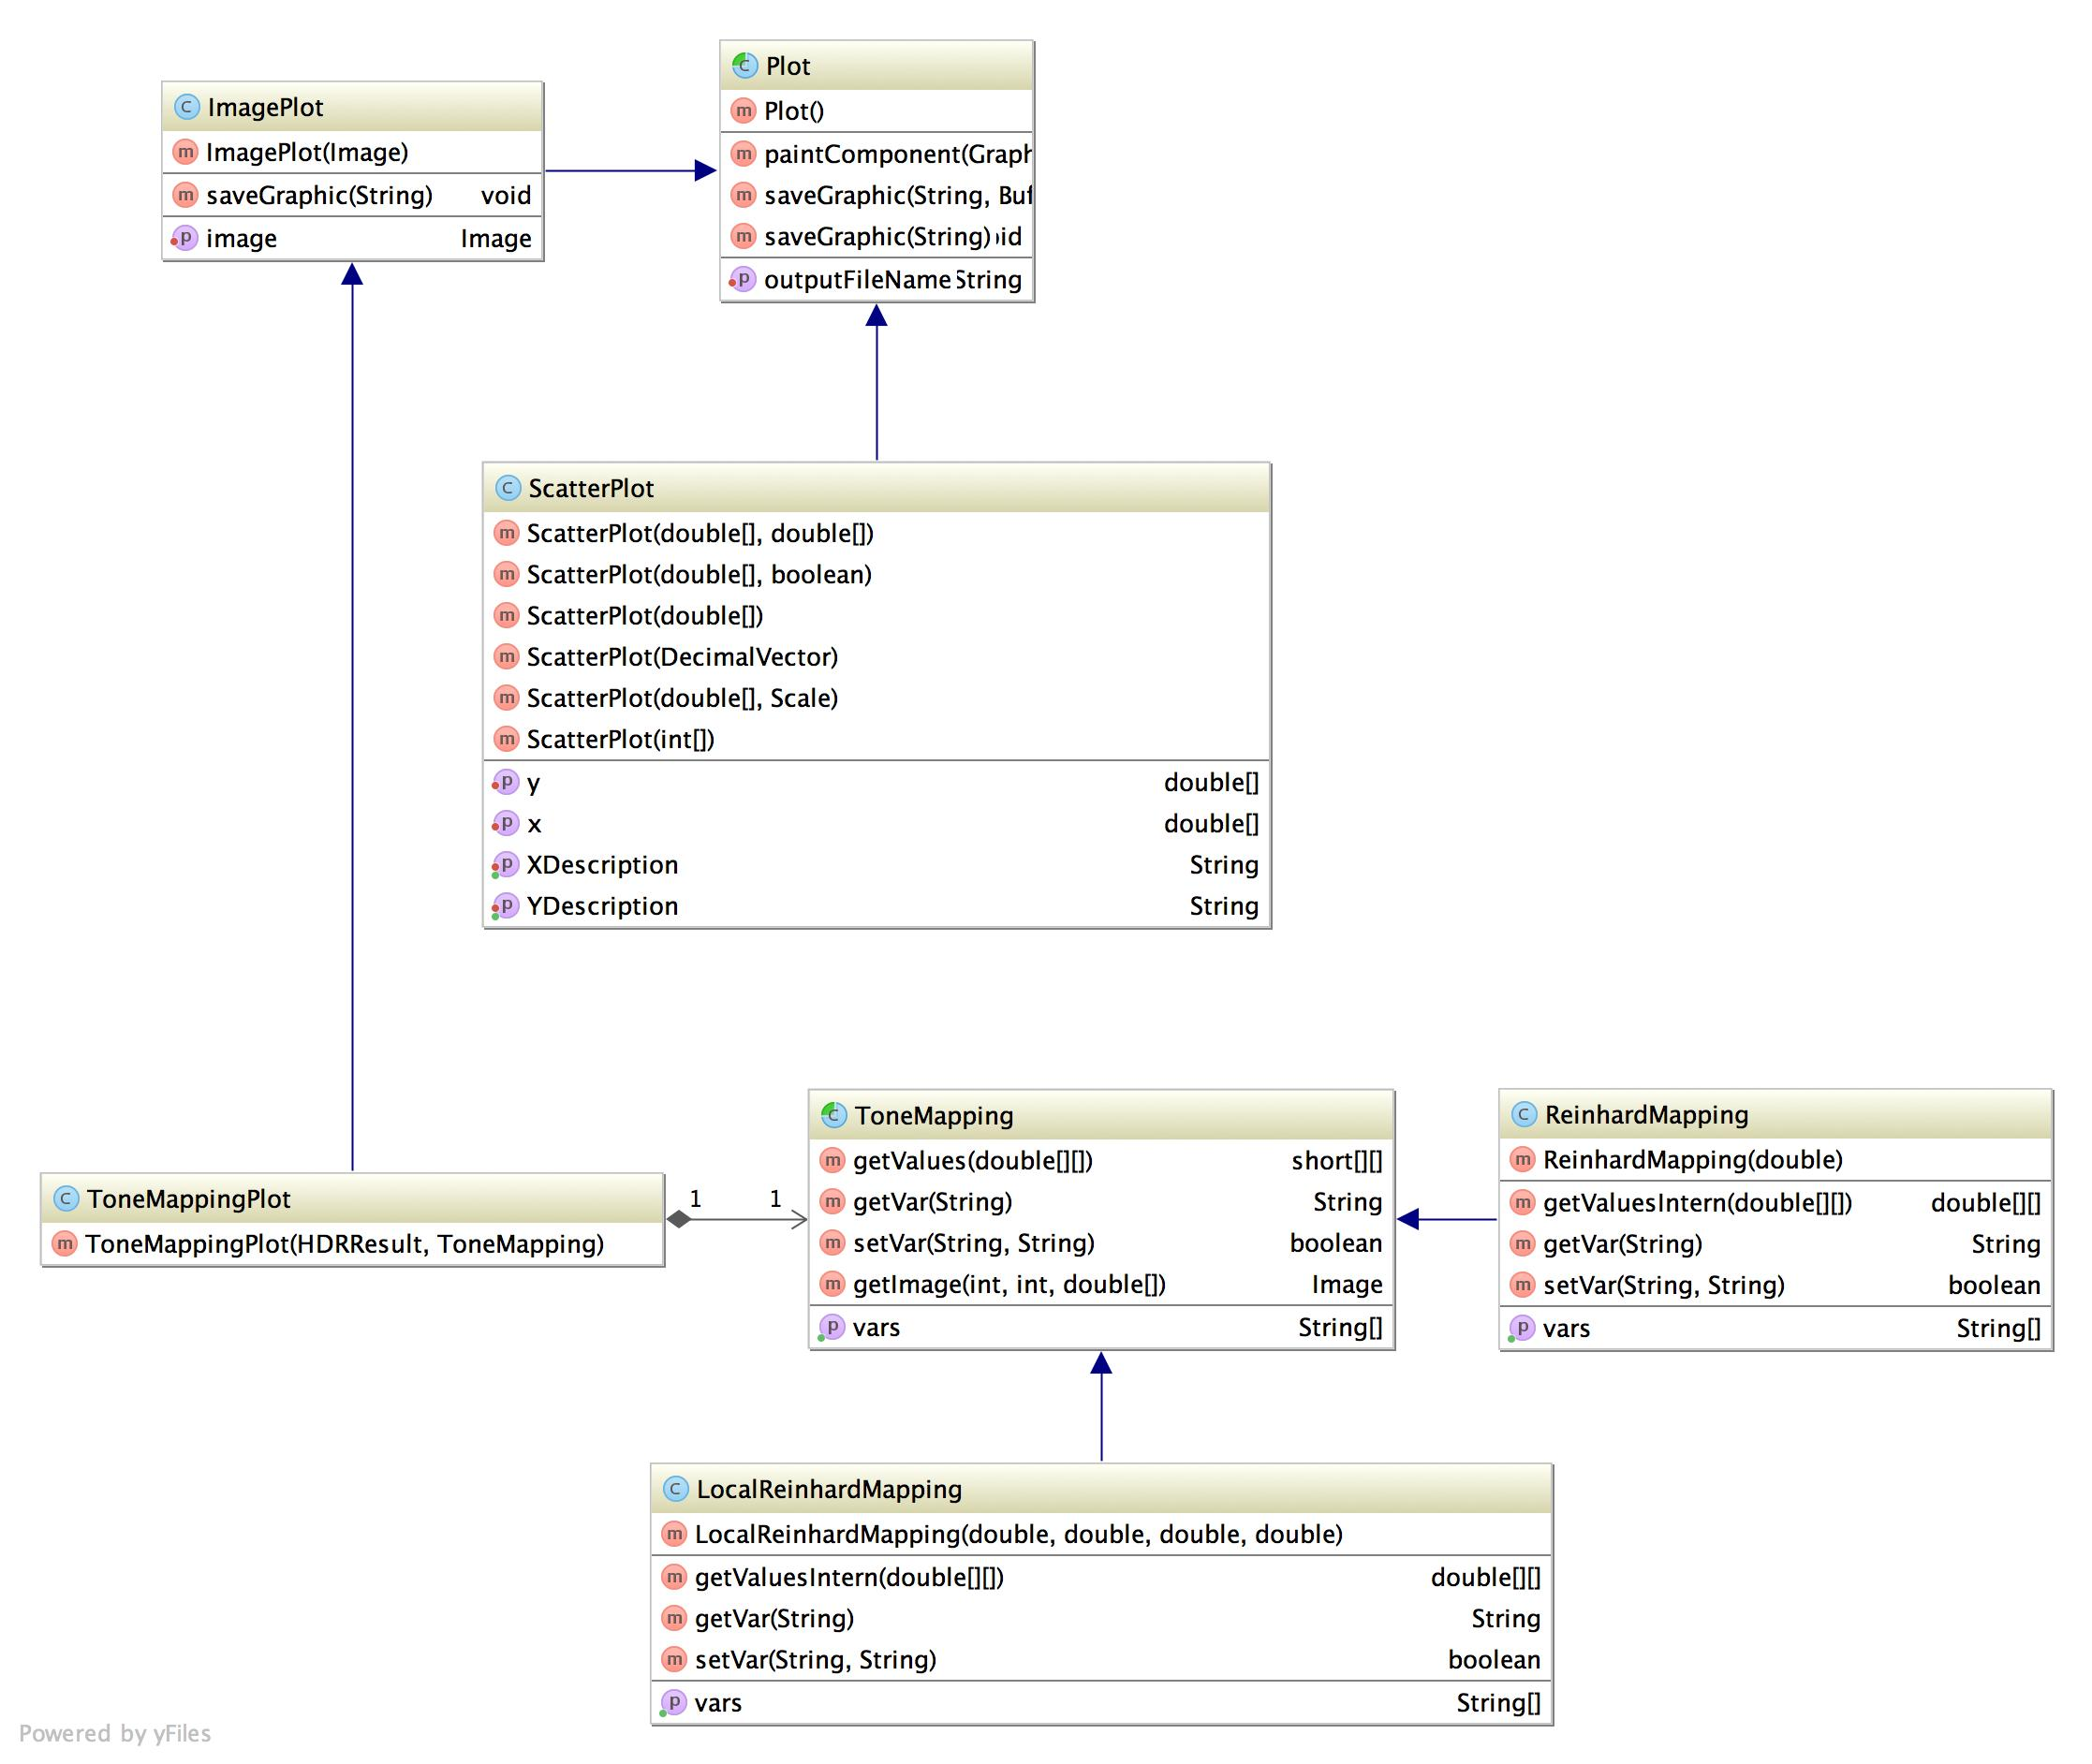
\includegraphics[width=0.8\textwidth]{architecture/plots}
    \caption{Die Struktur der verschiedenen grafischen Plots. Die Implementierungen von verschiedenen \gls{Tone-Mapping} Operatoren mittels Vererbung kann hier gut erkannt werden.}
    \label{fig:arch:plots}
  \end{center}
\end{figure}


\begin{figure}[H]
  \begin{center}
    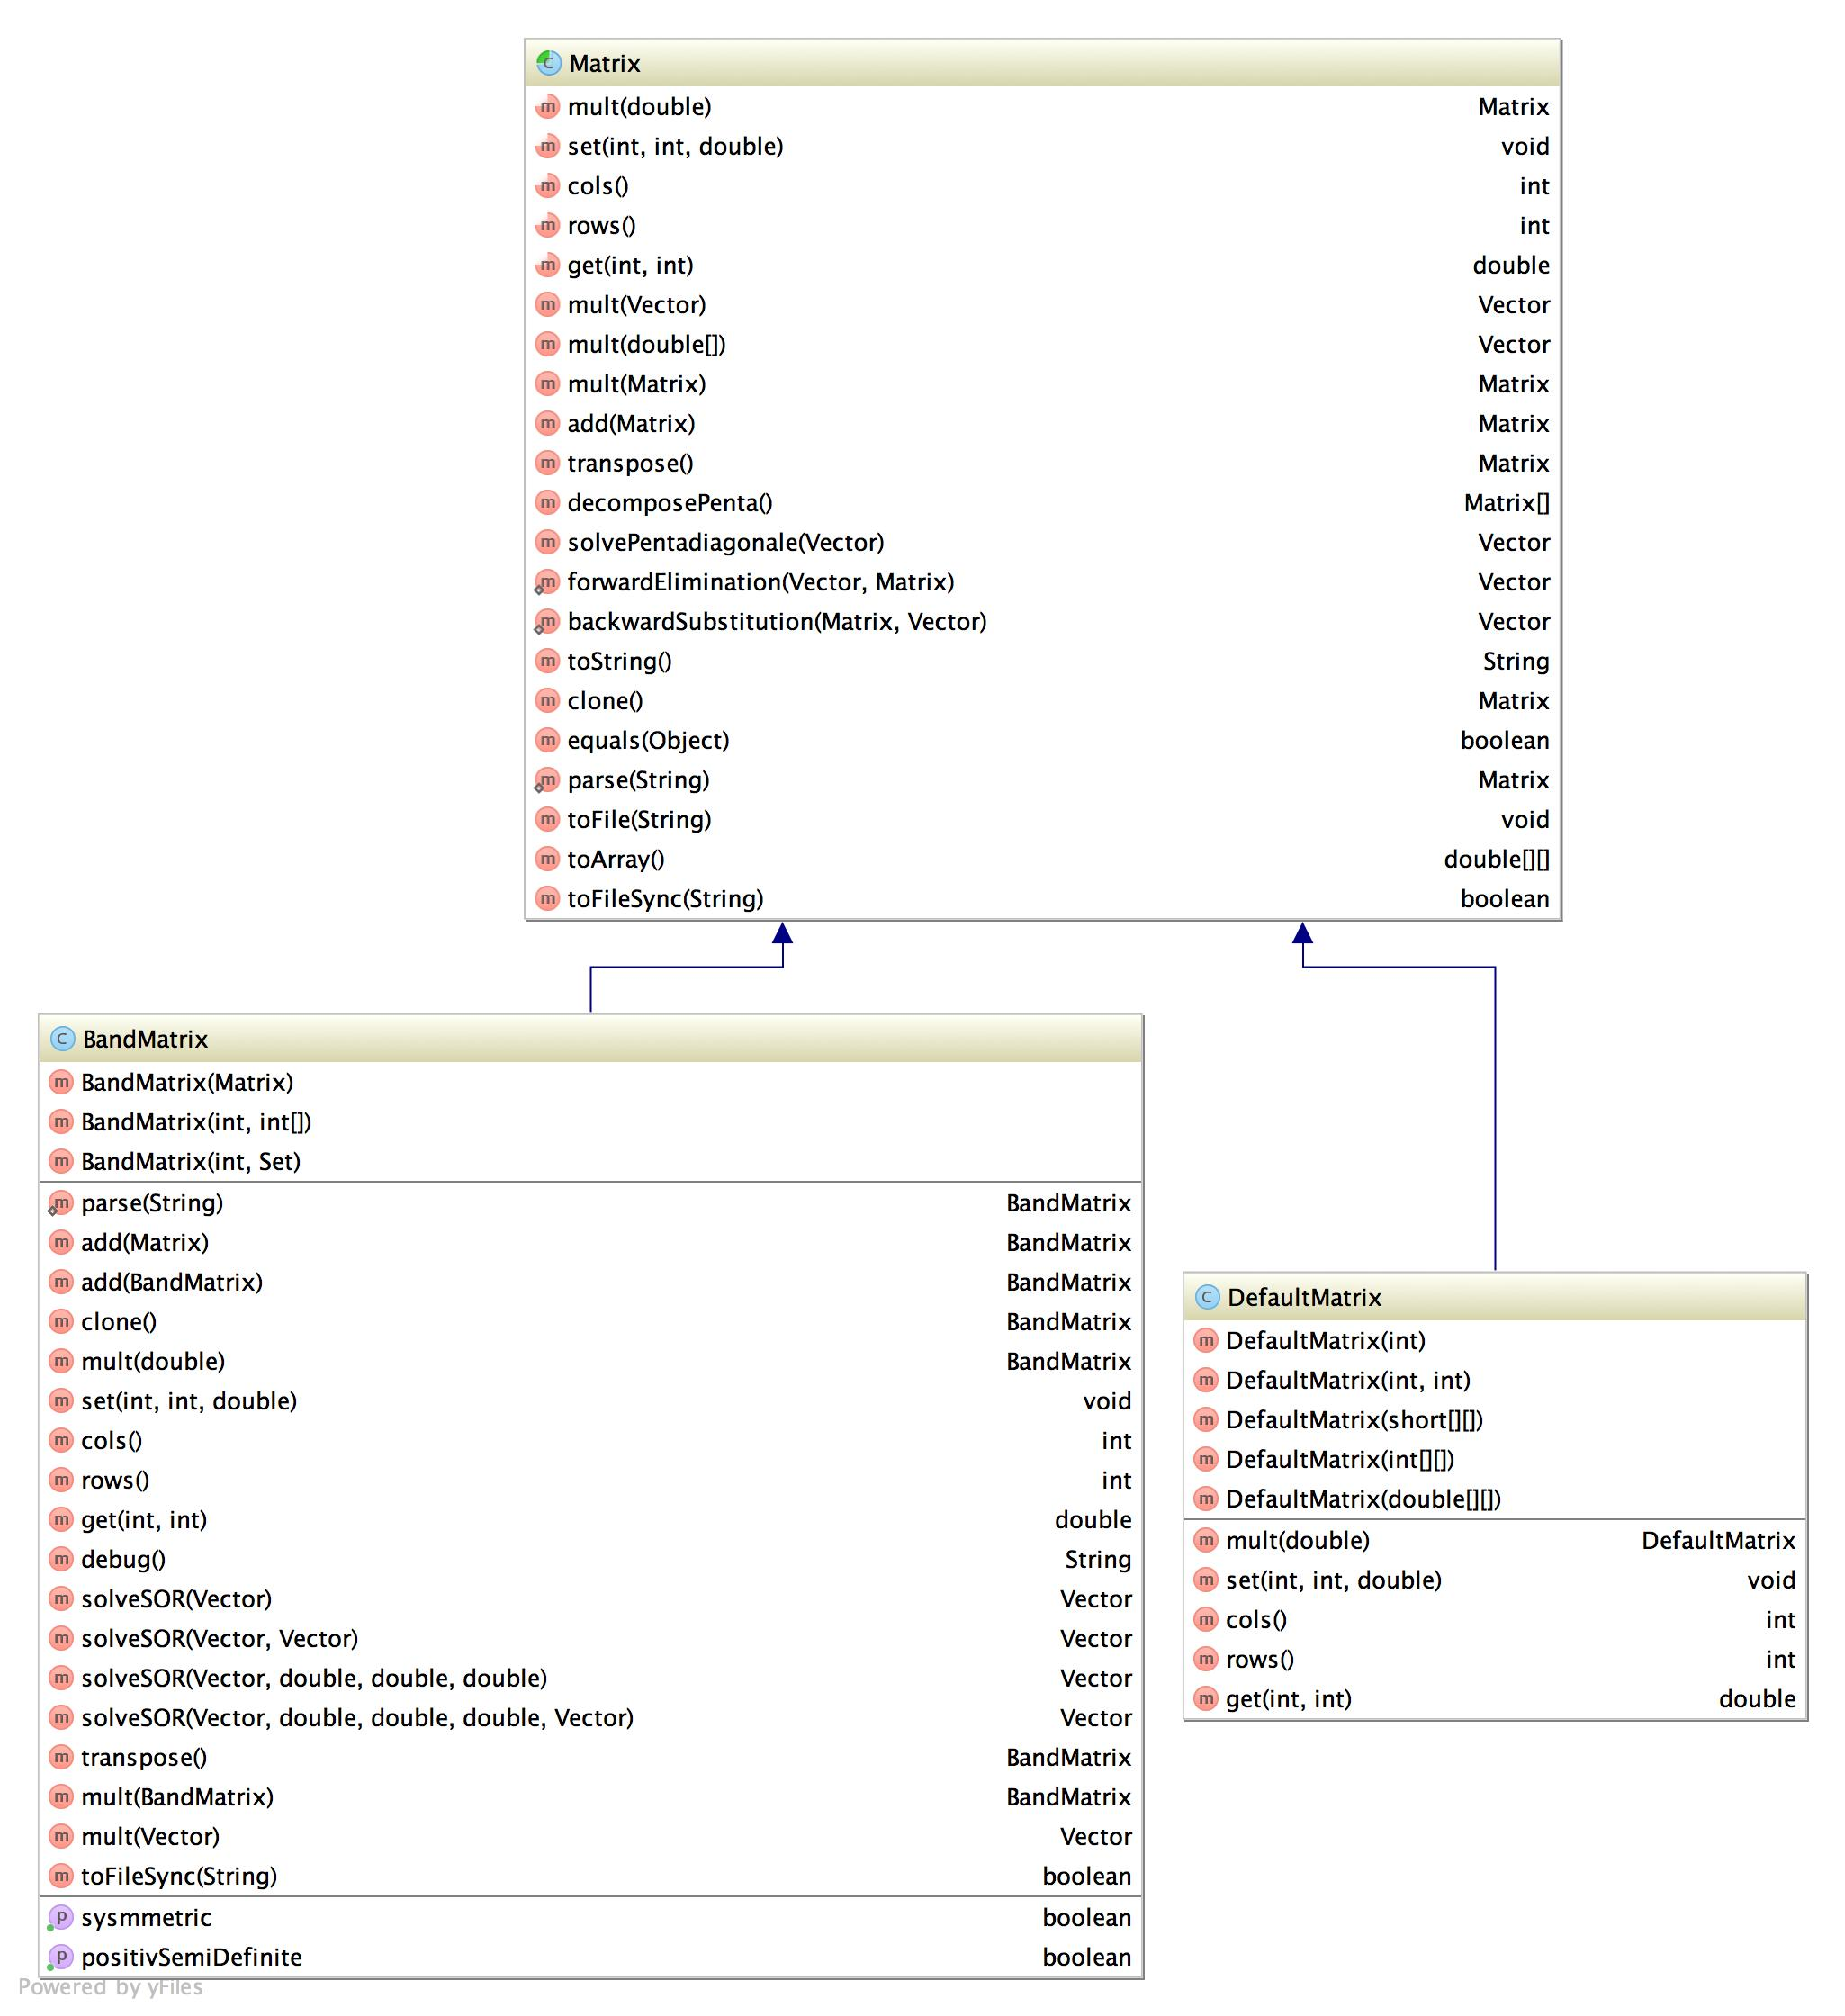
\includegraphics[width=\textwidth]{architecture/matrixes}
    \caption{Die Klasse \texttt{Matrix} und ihre Spezialisierungen \texttt{BandMatrix} und \texttt{DefaultMatrix}. Diese beiden Klassen dienen zusammen mit \texttt{Vector} als ein Kernbestandteil der mathematischen Berechnungen dieses Programmes.}
    \label{fig:arch:plots}
  \end{center}
\end{figure}


\subsection{Sequenzdiagramm}
Das Programm läuft sehr vielschichtig ab. Als grundsätzliche Architekturüberlegung stand jedoch zu Beginn der Aufbau wie in \autoref{fig:arch:sequence} beschrieben ist. Wichtig dabei ist, dass die grafische Benutzeroberfläche nicht von der Berechnungsdauer des Algorithmus blockiert wird, weshalb besonders zwischen \texttt{Controller} und \texttt{GUIFrame} asynchrone Methodenaufrufe zum Einsatz kommen.
\begin{figure}[H]
  \begin{center}
    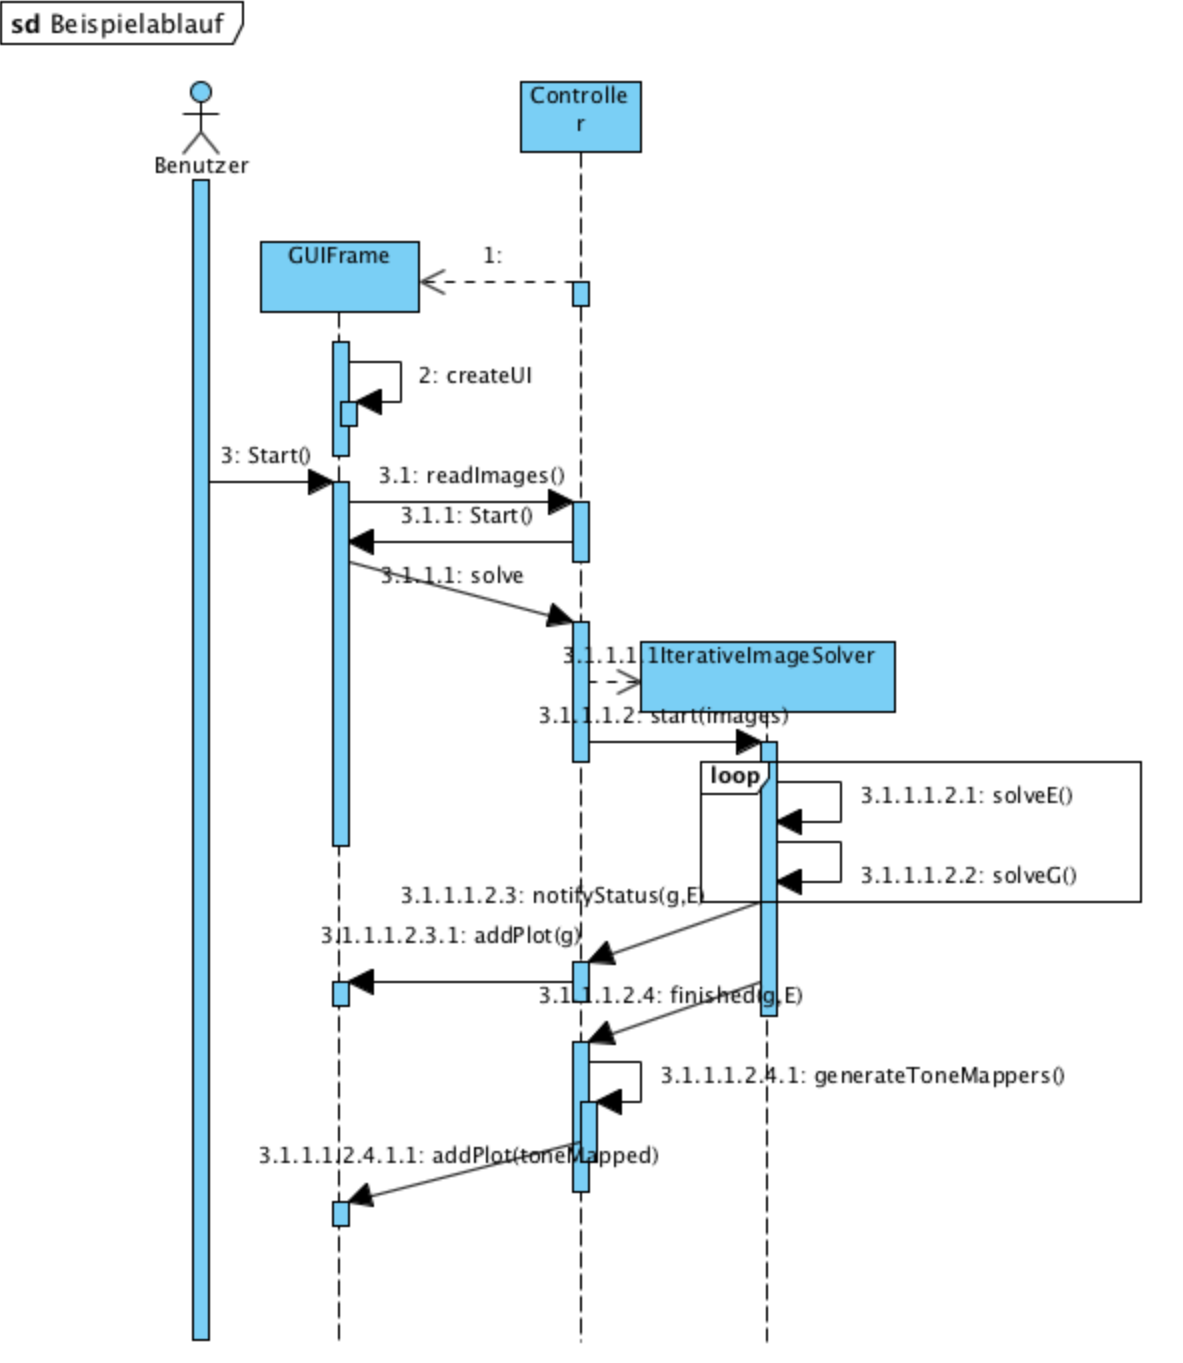
\includegraphics[width=0.8\textwidth]{architecture/sequence_example}
    \caption{Der grundsätzliche Ablauf der Berechnung des HDR-Bildes und der Antwortkurve und der dabei beteiligten Komponenten sowie deren Interaktion. }
    \label{fig:arch:sequence}
  \end{center}
\end{figure}

\section{Algorithmus in Pseudocode}
\label{sec:pseudocode}
\section{Ausgewählte Programmabschnitte}
\label{sec:sample-codes}
\section{Verwendetes \gls{Tone-Mapping}-Verfahren}
\label{sec:tone-mapping}
\section{Laufzeitanalyse}
\label{sec:laufzeit}


